% !TeX root = ../thuthesis-example.tex

\begin{translation}
\label{cha:translation}

\title{车队的队列稳定性:定义和分析方法}
\maketitle

% \tableofcontents

  \vspace{1em}
  \textbf{摘要:}由互相关联的自动驾驶车辆 (CAV) 组成的车队预计将对道路交通产生变革性影响,例如提高高速公路安全性、提高交通效率和减少燃料消耗。控制车队时的一项关键任务是实现队列稳定性(String Stability),
  为此提出了许多模型和算法。但是,尽管这些年来针对队列稳定性提出了许多不同的定义和分析方法,但是没有进行详尽的比较。 为了填补这些空白,本文旨在阐明这些模糊的定义与各种分析方法之间的关系,为今后的研究提供一个坚实
  的基础。本文总结和讨论了一系列等价的定义和算法,也讨论了不同分析方法和定义的优、缺点。 所有这些讨论为在实际使用中选择车队的分析方法提供了见解。

\section{引言}

  作为一种提高交通效率的有效方式,车队控制引起了广泛的兴趣。(Guanetti, Kim, and Borrelli, 2018; Horowitz and Varaiya, 2000; Ioannou and Chien,1993; Li, Zheng, Li, and Wang, 2015; Sheikholeslam and Desoer, 1990; Shladover, 1995)
  在一个车队中,由两辆及以上车辆组成的车队按照预先设置的巡航速度和车间距行驶。与人工驾驶相比,自动驾驶车队有着车与车之间的距离更小的优点(即队形更加紧密),被认为是一个很有希望的降低交通阻塞、空气阻力和燃油损耗的方法。
  (Al Alam, Gattami, and Johansson, 2010; Chien and Ioannou, 1992; Liand Chen, 2017)
  
  车队的紧密编队控制有一个特殊的困难,称为“队列不稳定性”,即系统中的扰动沿着车队不断放大,如图~\ref{fig:appendix-translation-figure1}(b)所示(参见Peppard(1974))。 
  正如观察 (Treiterer and Myers, 1974) 和实验 (Sugiyama et al., 2008) 所证明的那样,紧密编队车队的队列不稳定性会导致在环形线路和高速公路上出现没有瓶颈的堵塞(例如,走走停停),这严重损害了车队控制的好处。

\begin{figure}
  \centering
  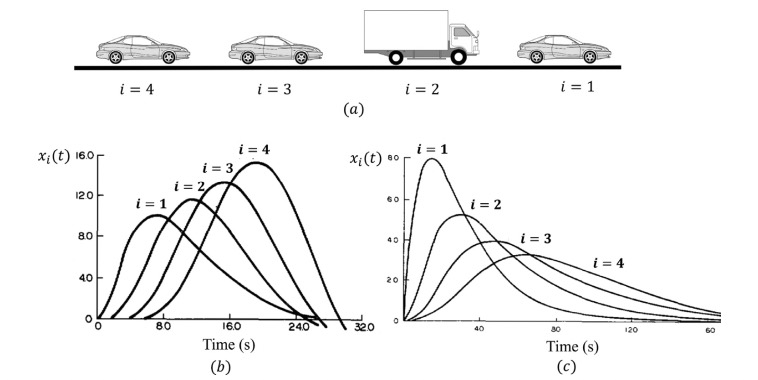
\includegraphics[width=1\linewidth]{appendix-A-1.jpg}
  \caption{车队系统图示(a)和队列稳定性的直观描述(b-c)(Peppard, 1974),其中$x_i(t)$表示车辆$i$在时间$t$的状态波动(例如位置误差)。}
  \label{fig:appendix-translation-figure1}
\end{figure}
   
  为了解决这个问题,队列稳定性的性质已经被广泛研究并应用于车队控制。直观地说,如果一个车队具有以下特性,则称它是队列稳定的,即扰动不会沿着车队被不断放大(Peppard,1974),
  如图~\ref{fig:appendix-translation-figure1}(c)所示。研究队列稳定性的基本过程可分为三个步骤:(1)数学上定义队列稳定性的性质;(2)根据分析方法推导出充分条件;(3) 设计控制器以满足充分条件

\subsection{研究动机}

  大量文献提出了很多种不同的的定义和分析方法。在许多研究中,虽然仿真结果显示出与图~\ref{fig:appendix-translation-figure1}(c)相似的性质,但队列稳定性的性质存在令人困惑的差异。
  许多不同的定义是基于不同的域(例如频域和时域)和范数(例如$\mathcal{L_2}$、$\mathcal{L_p}$和$\mathcal{L_\infty}$)、强度(例如弱和强)。模棱两可的定义阻碍了不同研究之间的比较。
  需要对它们之间的关系进行严格的分析以帮助进一步研究的进行。此外,学者已经提出了许多分析方法并衍生了许多性质,它们的关系、利弊以及可以解决什么问题尚未得到太多讨论。
  更好地理解这些方法和性质是进一步研究困难问题的基础。

\subsection{研究范围和目的}

本文重点介绍队列稳定性的定义和推导队列稳定性质的分析方法。为了更好地解释相关概念,我们将简要介绍一些车队控制的研究工作。然而,为了简明扼要,本文将不讨论车队控制领域的其他问题。
(Li et al., 2015; Li, Zheng et al., 2017)。

本文的目的是:(1)阐明队列稳定性模糊定义之间的关系,提出统一的定义; (2)讨论各种分析方法的关系、利弊、可以解决什么问题,并针对存在的棘手问题提出方法建议;(3)深入研究各性质之间的关系,
这为解决队列不稳定的问题提供了思路。

\subsection{主要贡献}

  本工作的主要贡献为:

  第一,严格分析了模糊不清的定义之间的关系。对常用的定义进行了介绍和比较。总结了队列稳定性的三个基本属性,即收敛性、有界性和可扩展性。类似于控制理论中稳定性定义,
  本文提出了三种类型的队列稳定性定义作为不同定义之间的桥梁,即李雅普诺夫稳定性、输入-输出稳定性和输入-状态队列稳定性。定理1详细阐述了对这些队列稳定性定义的严格分析。
  受该定理的启发,建议将所提出的定义,即输入-状态队列稳定性 (ISSS)用于未来的研究。,并且给出了推荐ISSS的理由。本文扩展并深化了对该领域先前主要对定义的讨论。
  (Ploeg, Van De Wouw, and Nijmeijer, 2014; Stüdli, Seron, and Middleton, 2017)

  第二,本文对各种分析方法进行了比较,并对通过使用这些分析方法推导得到的性质进行了严格的分析。这些方法可以分为三类:时间域分析方法、$z$域分析方法和$s$域分析方法。
  带分析的问题可分为时间维度和空间维度。本文分别从两个维度讨论了这些分析方法的优缺点,在此基础上我们推荐了针对现有困难问题的方法。此外,在定理2中对推导得到的性质进行了严格分析,
  从中展现了这些性质以及常用研究队列系统的推荐定义(即ISSS)之间的关系。 并将解决队列不稳定的常用解决方法与“弱耦合性质”进行了比较。

\section{预备知识}
  记实数域为$\mathbb{R}$,自然数集$\mathbb{N}={1, 2, \dots}$,对于向量$\chi \in \mathbb{R}^n$,其$p$范数为
  \begin{equation}
    \Vert\chi\Vert_p = \left( \sum_{i=1}^n{|\chi_i|^p} \right) ^{1/p}, p \in [1, \infty)
    \label{eq:appendix-equation-1}
  \end{equation}
  \begin{equation}
    \Vert\chi\Vert_\infty = \max_{i} |\chi_i|.
    \label{eq:appendix-equation-2}
  \end{equation}
  对于一个勒贝格可测的信号$\chi(t):I \rightarrow \mathbb{R}^n$,其$\mathcal{L}_p$范数$\Vert\chi\Vert^I_{\mathcal{L}_p}$定义为
  \begin{equation}
    \Vert\chi\Vert^I_{\mathcal{L}_p} = \left( \int_I{\Vert\chi\Vert_p^p dt} \right) ^{1/p} < \infty, p \in [1, \infty)
    \label{eq:appendix-equation-3}
  \end{equation}
  \begin{equation}
    \Vert\chi\Vert^I_{\mathcal{L}_\infty} = \sup_{t \in I} \Vert\chi\Vert_\infty,
    \label{eq:appendix-equation-4}
  \end{equation}
  当$I=[0, \infty)]$时,$\Vert\chi\Vert^{[0, \infty)]}_{\mathcal{L}_\infty}$简记为$\Vert\chi\Vert_{\mathcal{L}_\infty}$。给定一个系统的传递函数$G(j\omega)$,系统的$\mathcal{H}_\infty$范数定义为
  \begin{equation}
    \Vert G \Vert_{\mathcal{H}_\infty} = \sup_{\omega}|G(j\omega)|, {\rm (SISO)}
    \label{eq:appendix-equation-5}
  \end{equation}
  \begin{equation}
    \Vert G \Vert_{\mathcal{H}_\infty} = \sup_{\omega}\bar{\sigma} \left( G(j\omega) \right), {\rm (MIMO)}
    \label{eq:appendix-equation-6}
  \end{equation}
  SISO代表单输入单输出系统,MIMO代表多输入多输出系统。$\bar{\sigma} \left( G(j\omega) \right)$是矩阵$G(j\omega)$的最大奇异值(参见Zhou, Doyle, Glover et al., 1996)。
  对于连续函数$\alpha:[0, a) \rightarrow [0, \infty), a \in \mathbb{R}^+$,如果在其定义域上是严格单调递增的,并且$\alpha(0) = 0$,那么我们称这个函数是$\mathcal{K}$类函数。
  对于连续函数$\beta:[0, a) \times [0, \infty) \rightarrow [0, \infty)$,如果对于每一个固定的$s$,函数$\beta(\cdot, s)$是$\mathcal{}$类函数,并且对于每一个固定的$r$,函数$\beta(r, \cdot)$
  在其定义域上是单调递减的,且满足当$s \rightarrow 0$时,$\beta (r, s) \rightarrow 0$,那么我们称这个函数是$\mathcal{KL}$类函数。如果$\Vert\chi\Vert_{\mathcal{L}_\infty} < \infty$,我们
  称$\chi \in \mathcal{L}_\infty$。

  通常,我们考虑一个车队
  \begin{equation}
    \dot{\chi} = f(\chi, \omega),
    \label{eq:appendix-equation-7}
  \end{equation}
  \begin{equation}
    y = g(\chi)
  \end{equation}

  这里,函数$f(\chi, \omega): \mathbb{R}^{mn} \times \mathbb{R}^m \rightarrow \mathbb{R}^{mn}$是连续可导且全局Lipschitz的,
  函数$g(\chi): \mathbb{R}^{mn} \rightarrow \mathbb{R}^{m}$是连续可导且全局Lipschitz的。$\chi \in \mathbb{R}^{mn}$代表系统状态向量,
  $\omega \in \mathbb{R}^m$代表扰动。我们假设原点$\chi = 0$是非受迫系统$\dot{\chi} = f(\chi, 0)$的一个稳定平衡点。对于车队,$m \in \mathbb{N}$
  代表了车队长度,$n \in \mathbb{N}$代表子系统的状态阶数,表\ref{tab:appendix-translation-table1}列出了这些符号的含义。

  \begin{table}
    \centering
    \caption{所用变量的符号}
    \begin{tabular}{ll}
      \toprule
      变量          & 符号                        \\
      \midrule
      $S_m$           & $S_m = \{0\} \cup \{i \in \mathbb{N} | 1 \leqslant i \leqslant m-1 \}.$ \\
      $S_{e,m}$       & $S_m = \{i \in \mathbb{N} | 1 \leqslant i \leqslant m-1 \}.$                     \\
      $\chi_i(t)$     & $\chi_i(t) \in \mathbb{R}^n$代表第$i$个子系统的状态   \\
      $\omega_i(t)$   & $\omega_i(t) \in \mathbb{R}$代表第$i$个子系统受到的扰动 \\
      $y_i(t)$        & $y_i(t) \in \mathbb{R}$代表第$i$个子系统的输出        \\
      $\chi_i(t)$     & $\chi_i(t) \in \mathbb{R}^{mn}$代表系统的状态        \\
      $\omega(t)$     & $\omega(t) \in \mathbb{R}^m$代表系统受到的扰动        \\
      $y(t)$          & $y(t) \in \mathbb{R}^m$代表系统的输出        \\
      $\Chi_i(s), Y_i(s), U_i(s)$   & $\chi_i(t), y_i(t), u_i(t)$的拉普拉斯变换        \\
      $\Chi(s), Y(s), U(s)$         & $\chi(t), y(t), u(t)$的拉普拉斯变换        \\
      $\mathcal{\Chi}(z), \mathcal{Y}(z), \mathcal{U}(z)$   & $\chi(t), y(t), u(t)$的$z$变换        \\
      \bottomrule
    \end{tabular}
    \label{tab:appendix-translation-table1}
  \end{table}


\section{车队控制}

本节简要介绍了车队的控制问题,该问题引发了对队列稳定性的研究。车队的控制问题最初由Levine和Athans于1966年提出,研究如何设计一个控制器来实现队列系统的控制。
这包括队列系统描述、控制目标和控制器设计方法。并且介绍了本文的两个重点的背景,即队列稳定性的定义和分析方法。

\subsection{队列系统描述}

车队系统的描述确定了队列稳定问题的研究场景。本文采用了由四个部分组成的框架(Li et al., 2015),即节点动力学、信息流拓扑结构、分布式控制和队形几何。
此外,还强调了系统的通信质量和收到的干扰。一个特定的车队系统可以通过这六个部分来唯一确定,本小节中用到的缩写在表A.1中列出。


\appendix

\section{缩写表}

\begin{table}
  \centering
  \caption{对车队系统的描述的缩写}
  \begin{tabular}{ll}
    \toprule
    变量          & 符号                        \\
    \midrule
    $S_m$           & $S_m = \{0\} \cup \{i \in \mathbb{N} | 1 \leqslant i \leqslant m-1 \}.$ \\
    $S_{e,m}$       & $S_m = \{i \in \mathbb{N} | 1 \leqslant i \leqslant m-1 \}.$                     \\
    $\chi_i(t)$     & $\chi_i(t) \in \mathbb{R}^n$代表第$i$个子系统的状态   \\
    $\omega_i(t)$   & $\omega_i(t) \in \mathbb{R}$代表第$i$个子系统受到的扰动 \\
    $y_i(t)$        & $y_i(t) \in \mathbb{R}$代表第$i$个子系统的输出        \\
    $\chi_i(t)$     & $\chi_i(t) \in \mathbb{R}^{mn}$代表系统的状态        \\
    $\omega(t)$     & $\omega(t) \in \mathbb{R}^m$代表系统受到的扰动        \\
    $y(t)$          & $y(t) \in \mathbb{R}^m$代表系统的输出        \\
    $\Chi_i(s), Y_i(s), U_i(s)$   & $\chi_i(t), y_i(t), u_i(t)$的拉普拉斯变换        \\
    $\Chi(s), Y(s), U(s)$         & $\chi(t), y(t), u(t)$的拉普拉斯变换        \\
    $\mathcal{\Chi}(z), \mathcal{Y}(z), \mathcal{U}(z)$   & $\chi(t), y(t), u(t)$的$z$变换        \\
    \bottomrule
  \end{tabular}
  \label{tab:appendix-translation-table1}
\end{table}


% 书面翻译的参考文献
\bibliographystyle{unsrtnat}
\bibliography{ref/appendix}

% 书面翻译对应的原文索引
\begin{translation-index}
  \nocite{salomon1995advanced}
  \bibliographystyle{unsrtnat}
  \bibliography{ref/appendix}
\end{translation-index}

\end{translation}
